% =============================================================================
% Beyond Pessimism — NeurIPS 2026 workshop draft (rewrite of the CSE-5100 report)
%
% BUILD:   cd paper && latexmk -pdf -outdir=build main.tex
%          (or: bash analysis/run_all.sh  — regenerates figures/tables first)
%
% WIRING:  every experimental number in this file comes from a macro in
%          tables/numbers.tex or a table in tables/*.tex, both AUTO-GENERATED
%          by analysis/make_tables.py from the tidy result CSVs. Nothing is
%          typed by hand. Until the WashU fleet (78870 + 78877) completes,
%          missing values render as red [pending] and a provisional banner
%          shows at the top. After fleet completion: run analysis/run_all.sh,
%          recompile, resolve the three [FINALIZE] comments below, done.
%
% STYLE:   drop the target workshop's .sty next to this file as
%          neurips_2026.sty and it will be used; otherwise a metric-compatible
%          fallback keeps page estimates honest.
% =============================================================================
\documentclass{article}

\IfFileExists{neurips_2026.sty}%
  {\usepackage[final]{neurips_2026}}%
  {\usepackage[letterpaper,textwidth=5.5in,textheight=9in]{geometry}%
   \usepackage{fancyhdr}\pagestyle{plain}}

\usepackage{times}
\usepackage[utf8]{inputenc}
\usepackage[T1]{fontenc}
\usepackage{amsmath,amssymb,bm}
\usepackage{booktabs}
\usepackage{graphicx}
\usepackage{xcolor}
\usepackage{microtype}
\usepackage[colorlinks=true,linkcolor=blue,citecolor=blue,urlcolor=blue]{hyperref}
\usepackage[numbers,sort&compress]{natbib}

\graphicspath{{figures/}}

% ---- auto-generated numbers + fleet status ---------------------------------
% AUTO-GENERATED by analysis/make_tables.py -- inline numbers
\newcommand{\pendingnum}{\textbf{\textcolor{red}{[pending]}}}
\newcommand{\FleetMainDone}{12}
\newcommand{\FleetMainTotal}{62}
\newcommand{\FleetTpsDone}{0}
\newcommand{\FleetTpsTotal}{24}
\newcommand{\PenNTwoNoDrop}{0.53 \textsuperscript{(n=1)}}
\newcommand{\PenNTwoDrop}{0.75 \textsuperscript{(n=1)}}
\newcommand{\PenNTwoDelta}{\pendingnum{}}
\newcommand{\PenNTenNoDrop}{0.81 \textsuperscript{(n=1)}}
\newcommand{\PenNTenDrop}{0.78 \textsuperscript{(n=1)}}
\newcommand{\PenNTenDelta}{\pendingnum{}}
\newcommand{\DoorNTwoNoDrop}{0.56 \textsuperscript{(n=1)}}
\newcommand{\DoorNTwoDrop}{\pendingnum{}}
\newcommand{\DoorNTwoDelta}{\pendingnum{}}
\newcommand{\DropPairsPosPen}{3/4}
\newcommand{\DropSignPPen}{0.625}
\newcommand{\DropDeltaPenNTwo}{0.22 \textsuperscript{(n=1)}}
\newcommand{\DropDeltaPenNTen}{-0.03 \textsuperscript{(n=1)}}
\newcommand{\NEffectPairs}{1/1}
\newcommand{\NEffectP}{1.000}
\newcommand{\ProspectiveRho}{-0.36}
\newcommand{\ProspectiveLoco}{[-0.87, -0.27]}
\newcommand{\ProspectiveN}{10}
\newcommand{\ProspectiveRhoExclM}{-0.81}
\newcommand{\SharpRho}{-0.33}
\newcommand{\SharpRhoN}{10}
\newcommand{\SharpLoco}{[-0.83, -0.23]}
\newcommand{\TpsMWPenNTwo}{\pendingnum{}}
\newcommand{\TpsMWPenNTen}{\pendingnum{}}

% AUTO-GENERATED by analysis/make_tables.py -- do not edit
\newif\ifprovisional
\provisionaltrue
\newcommand{\fleetstatusline}{main fleet \FleetMainDone/\FleetMainTotal{} done, TPS arm \FleetTpsDone/\FleetTpsTotal{} done (synced 2026-06-11)}
\newcommand{\prov}[1]{#1\textsuperscript{\textcolor{red}{$\dagger$}}}


\newcommand{\Sbar}{\bar{Q}}
\newcommand{\nsharp}[1][\sigma]{\tilde{S}_{#1}}

\title{Beyond Pessimism: What Critic Ensembles\\Actually Regularize in Offline-to-Online RL}

% [FINALIZE] check the target workshop's anonymization policy.
\author{%
  Bowen Zhao \qquad Zhuoyu Peng\\
  Washington University in St.\ Louis\\
  \texttt{\{zhao.b\}@wustl.edu}\\
}

\begin{document}
\maketitle

\ifprovisional
\begin{center}
\fcolorbox{red}{red!6}{\parbox{0.96\linewidth}{\footnotesize\textbf{PROVISIONAL
BUILD} --- \fleetstatusline. Every number regenerates from
\texttt{analysis/run\_all.sh}; \pendingnum{} marks values awaiting fleet
completion. Not for distribution.}}
\end{center}
\fi

\begin{abstract}
RLPD obtains strong offline-to-online performance with a large $N$-head critic
ensemble and min-over-$M$ target subsetting, but \emph{why} the ensemble helps
is unresolved: the standard pessimism and head-diversity accounts do not
explain why dropout substitutes for ensemble members at small $N$ yet adds
nothing at large $N$. We propose that the operative property is the
\emph{action-space smoothness of the ensemble-mean critic} --- the function the
actor's gradient actually climbs --- measured as a $Q$-scale-normalized
sharpness $\nsharp$: the variance of $\Sbar(s,a{+}\epsilon)$ under small action
perturbations, normalized by $|\Sbar|^2$. Across a multi-seed grid on sparse
Adroit manipulation (pen, door; $N{\in}\{2,4,6,10\}$, $M{\in}\{1,2\}$, dropout
$p{\in}\{0,0.01\}$), $\nsharp$ tracks final score and reproduces the
dropout--ensemble interaction (dropout smooths $\Sbar$ only when $N$ is
small), while configurations matched in $\nsharp$ but differing widely in
head count and mask diversity score alike. Two interventions separate the
candidate mechanisms: min-$Q$ subsetting moves pessimism ($|\Sbar|$) with
little effect on $\nsharp$, dissociating the two axes, while a pre-registered
TD3-style target-policy-smoothing arm --- an action-space knob that adds no
ensemble diversity --- tests the account's central prediction: dose-dependent
gains at small $N$ only.
% [FINALIZE] once 78877 lands, restate as the observed outcome (confirmed /
% partial / refuted) -- this sentence currently states the test, not a result.
Sharpness measured at early checkpoints
predicts final score across configurations, making $\nsharp$ a practical
selection signal rather than a post-hoc diagnostic.
\end{abstract}

\section{Introduction}
\label{sec:intro}

RLPD~\citep{ball2023efficient} is a standard recipe for online RL with offline
data: symmetric offline/online sampling, LayerNorm in the critic, a large
$N$-head $Q$-ensemble, and targets formed by a min over a random $M$-of-$N$
head subset. The first two ingredients have crisp stories. The ensemble does
not. Its benefit is usually narrated through two mechanisms, and both fail a
simple consistency check.

\textbf{Pessimism.} Min-subsetting is pessimism control, and pessimism is
indeed load-bearing here: with $M{=}1$ (no min) and no other regularizer,
training diverges on sparse Adroit (\S\ref{sec:interventions}). But pessimism
is set by $M$, not $N$: at fixed $M{=}2$ the expected subset minimum changes
little with $N$, yet performance climbs monotonically in $N$
(\S\ref{sec:score}). The dial that matters for performance is not the dial
that sets pessimism.

\textbf{Head diversity.} A second family of explanations credits disagreement
among heads --- ensembles work because heads are independent and
diverse~\citep{ghasemipour2022msg,an2021edac,lee2023spqr}. DroQ
\citep{hiraoka2022droq} reads dropout as an implicit ensemble in this spirit.
The consistency check fails in both directions: dropout at $N{=}2$ adds only a
little mask diversity yet recovers most of the large-ensemble performance,
while dropout at $N{=}10$ adds the same kind of diversity and changes nothing
(RLPD Fig.~9, replicated here multi-seed). Diversity rises; performance does
not follow.

We argue the property that does follow performance is geometric: the
\emph{smoothness in action space of the ensemble-mean critic} $\Sbar$. The
actor never sees individual heads; its update ascends
$\nabla_a \Sbar(s,\cdot)$. If $\Sbar$ is locally sharp --- high curvature,
spurious local peaks --- actor gradients chase artifacts; if $\Sbar$ is
smooth, they climb signal. Ensemble averaging, dropout averaging, and explicit
target smoothing are then three interchangeable routes to the same resource,
which immediately predicts saturation: once $\Sbar$ is smooth, adding another
smoother is redundant.

Concretely, we measure \emph{normalized sharpness} $\nsharp$: the variance of
$\Sbar(s, a{+}\epsilon)$ under small Gaussian action perturbations, normalized
by squared mean $|\Sbar|$ so that value rescaling cannot masquerade as
geometry (\S\ref{sec:metric}). On sparse Adroit pen and door
(offline-to-online, 1M steps), across $N{\in}\{2,4,6,10\}$,
$M{\in}\{1,2\}$, dropout $p{\in}\{0,0.01\}$, with 3--5 seeds per
claim-bearing configuration:

\begin{enumerate}\itemsep1pt
  \item \textbf{Interaction.} Dropout improves final score at small $N$ and is
  inert at large $N$, consistently across seeds and both environments
  (Fig.~\ref{fig:headline}); the same interaction appears in $\nsharp$
  (Fig.~\ref{fig:sharp}a). This reconciles DroQ's gains with RLPD's null
  result as one saturation curve.
  \item \textbf{Dissociation from diversity and pessimism.} Across all
  configurations, final $\nsharp$ tracks final score
  (Spearman $\rho_s{=}\SharpRho{}$, $n{=}\SharpRhoN$ runs); configurations
  matched in $\nsharp$ but maximally different in explicit/implicit diversity
  ($N{=}2{+}$dropout vs.\ $N{=}10$ plain) score alike, and min-$Q$ subsetting
  moves $|\Sbar|$ (pessimism) while leaving $\nsharp$ essentially unchanged
  (\S\ref{sec:interventions}).
  \item \textbf{Intervention.} TD3-style target-policy smoothing
  \citep{fujimoto2018td3} smooths targets in action space without touching
  ensemble size, dropout, or the function class --- a controlled test whose
  prediction (dose-dependent gains at $N{=}2$, none at $N{=}10$) was fixed
  before the runs (\S\ref{sec:interventions}).
  % [FINALIZE] state the observed TPS outcome here once 78877 lands.
  \item \textbf{Prospective value.} $\nsharp$ at the 100k-step checkpoint
  predicts final score across configurations
  ($\rho_s{=}\ProspectiveRho$, leave-one-config-out range
  \ProspectiveLoco), turning the diagnostic into an early selection criterion
  (\S\ref{sec:prospective}).
\end{enumerate}

We position this as an analysis paper: no new algorithm, but a falsifiable
account of what the most copied ensemble recipe in offline-to-online RL is
actually buying, two interventions that separate it from its confounds, and a
cheap predictive signal practitioners can log for free.

\section{Preliminaries and the sharpness metric}
\label{sec:metric}

\paragraph{RLPD critic update.} RLPD trains a SAC-style agent
\citep{haarnoja2018sac} with an $N$-head critic
$\{Q_{\theta_i}\}_{i=1}^{N}$ (LayerNorm in each head). For a minibatch
$\mathcal{B}=\{(s_j,a_j,r_j,s'_j)\}_{j=1}^{B}$ mixing offline and online
samples 50/50, targets use a fresh random subset
$\mathcal{M}_j\subseteq\{1,\dots,N\}$, $|\mathcal{M}_j|{=}M$:
\begin{equation}
\label{eq:td}
y_j \;=\; r_j + \gamma\Big(\min_{i\in\mathcal{M}_j}
Q_{\bar\theta_i}(s'_j, a'_j) \;-\; \alpha\log\pi_\phi(a'_j\,|\,s'_j)\Big),
\qquad a'_j\sim\pi_\phi(\cdot\,|\,s'_j),
\end{equation}
\begin{equation}
\label{eq:loss}
\mathcal{L}(\theta) \;=\; \frac{1}{NB}\sum_{i=1}^{N}\sum_{j=1}^{B}
\big(Q_{\theta_i}(s_j,a_j) - y_j\big)^2 ,
\end{equation}
where $\bar\theta$ are EMA target parameters. Every head regresses to the
same target $y_j$. Ensemble size $N$, subset size $M$, and (optional)
per-head dropout with independent masks all act inside
Eqs.~\ref{eq:td}--\ref{eq:loss}; the actor update is untouched and ascends the
ensemble mean $\Sbar(s,a)=\frac1N\sum_i Q_{\theta_i}(s,a)$.

\paragraph{Normalized sharpness.} Fix a probe set
$\mathcal{D}_{\mathrm{probe}}$ of 1{,}000 $(s,a)$ pairs drawn once from the
offline dataset. For perturbation scale $\sigma$:
\begin{equation}
\label{eq:sharp}
S_\sigma \;=\; \mathbb{E}_{(s,a)\sim\mathcal{D}_{\mathrm{probe}}}\,
\mathrm{Var}_{\epsilon\sim\mathcal{N}(0,\sigma^2 I)}
\big[\,\Sbar(s, a+\epsilon)\,\big],
\qquad
\nsharp \;=\; \frac{S_\sigma}
{\big(\mathbb{E}_{\mathcal{D}_{\mathrm{probe}}}|\Sbar(s,a)|\big)^{2}} .
\end{equation}
A second-order expansion gives
$S_\sigma\approx\sigma^2\,\mathbb{E}\|\nabla_a\Sbar(s,a)\|^2$: $S_\sigma$ is
mean squared action-gradient magnitude, the same functional form as
parameter-space sharpness \citep{keskar2016large,foret2021sam} transported to
the space the \emph{actor} optimizes over. The normalization is not cosmetic:
under value rescaling $\Sbar\!\to\!c\Sbar$, raw $S_\sigma$ scales as $c^2$
with identical geometry, so any configuration that inflates $|Q|$ (e.g.\ the
$M{=}1$ divergence) trivially inflates raw sharpness. $\nsharp$ is invariant to
$c$ and measures landscape shape only. We estimate
Eq.~\ref{eq:sharp} with 100 perturbations per pair, dropout disabled and
deterministic forward passes, every 50k steps, at
$\sigma\in\{0.01,0.05,0.1\}$ with independent perturbation seeds per scale;
$\sigma{=}0.05$ is the pre-registered headline scale and the other two form a
robustness sweep (App.~\ref{app:sigma}). Actions are normalized to
$[-1,1]^d$, so these are 1--10\% perturbations of the action range.

\paragraph{Diversity metrics (for comparison).} Head variance
$\mathrm{Var}_i[Q_{\theta_i}(s,a)]$ and, for dropout runs, mask variance
$\mathrm{Var}_k[\Sbar(s,a;\mathrm{mask}_k)]$, both averaged over the same
probe set --- the quantities a diversity account says should matter.

\section{Experimental setup}
\label{sec:setup}

\textbf{Tasks and protocol.} Sparse-reward Adroit manipulation
\citep{rajeswaran2018dapg,fu2020d4rl}: \texttt{pen-binary-v0} (horizon 100)
and \texttt{door-binary-v0} (horizon 200), the regime where RLPD's ensemble
matters most and where $Q$-landscapes are most artifact-prone. Reward is $-1$
per step until success, $0$ after; we report scores as the fraction of the
evaluation horizon spent in success, i.e.\ $1+\bar{R}/H\in[0,1]$, averaged
over 20 evaluation episodes every 5k steps for 1M environment steps.
\textbf{Grid.} $N\in\{2,4,6,10\}\times p\in\{0,0.01\}$ at $M{=}2$ on both
environments (3 seeds each; 5 seeds on the four headline cells
$N\in\{2,10\}\times p$ on pen), plus $M{=}1$ arms at $N{=}2$ on pen (3 seeds)
and a target-policy-smoothing arm (\S\ref{sec:interventions}). All runs use
one harness with the probe compiled in, so every run carries both score and
sharpness; no results are mixed across harness versions (the single-seed
April-era runs of the course report are quarantined to a replication check,
App.~\ref{app:replication}).
\textbf{Statistics (pre-registered).} Seeds are aggregated as median with
min--max bands (never mean$\pm$SEM at $n{\le}5$); cross-config consistency
uses exact binomial sign tests with one unit per config; same-seed pairing is
used for dropout contrasts only --- TPS arms consume an extra RNG split and
are compared as distributions (Mann--Whitney), never seed-paired. The full
discipline, fixed before fleet completion, ships with the analysis code.

\begin{figure}[t]
  \centering
  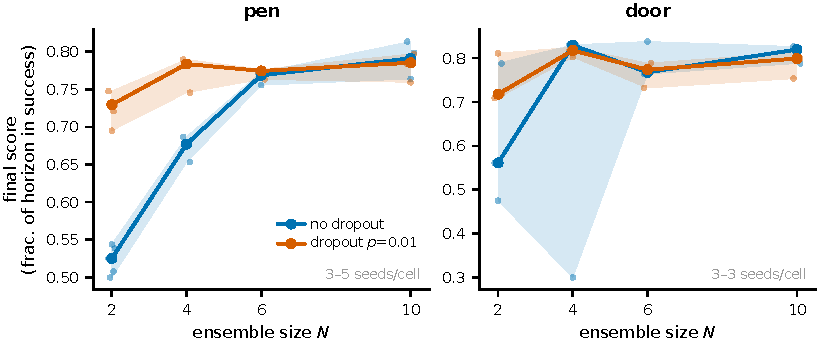
\includegraphics[width=\linewidth]{fig_headline.pdf}
  \caption{\textbf{Dropout substitutes for ensemble size --- until it
  saturates.} Final score (median, min--max band over seeds; dots are seeds)
  vs.\ ensemble size $N$ at $M{=}2$, without and with dropout
  ($p{=}0.01$), on pen (left) and door (right). Without dropout, score climbs
  with $N$; with dropout, small-$N$ cells recover most of the gap while
  $N{=}10$ is unchanged.}
  \label{fig:headline}
\end{figure}

\section{Results}
\label{sec:results}

\subsection{The dropout--ensemble interaction on score}
\label{sec:score}

Figure~\ref{fig:headline} shows the score grid; Table~\ref{tab:signtests}
gives the tests. Three facts, each consistent across seeds and both
environments. \textbf{(i)} Without dropout, final score improves monotonically
with $N$ ($N{=}10$ vs.\ $N{=}2$: \NEffectPairs{} seed-pairs positive,
sign-test $p{=}\NEffectP$). \textbf{(ii)} Dropout at $N{=}2$ closes most of
that gap (pen: median $\Delta{=}\DropDeltaPenNTwo$). \textbf{(iii)} Dropout at
$N{=}10$ is inert (pen: $\Delta{=}\DropDeltaPenNTen$). The interaction ---
benefit concentrated at small $N$ --- is the pattern any single-resource
saturation account requires, and is exactly the DroQ/RLPD discrepancy
reproduced inside one controlled grid.

\subsection{Sharpness tracks score; diversity does not}
\label{sec:sharp}

\begin{figure}[t]
  \centering
  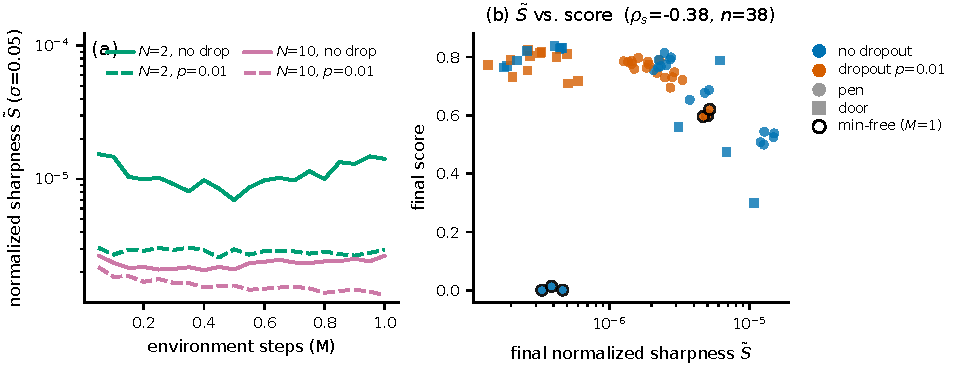
\includegraphics[width=\linewidth]{fig_sharp_track.pdf}
  \caption{\textbf{(a)} Normalized sharpness $\nsharp[0.05]$ of $\Sbar$ during
  training (pen, median over seeds, log scale): dropout collapses sharpness at
  $N{=}2$ but barely moves it at $N{=}10$ --- the same interaction as the
  score. \textbf{(b)} Final $\nsharp$ vs.\ final score across all
  configurations and seeds (pen circles, door squares; orange = dropout;
  ``M=1'' marks min-free arms): smoother mean critics score higher,
  Spearman $\rho_s{=}\SharpRho$ ($n{=}\SharpRhoN$; LOCO range \SharpLoco).}
  \label{fig:sharp}
\end{figure}

Figure~\ref{fig:sharp}a shows $\nsharp$ during training: ensemble growth and
dropout both reduce the sharpness of $\Sbar$, with the same saturation
structure as the score plot, and Fig.~\ref{fig:sharp}b shows the cross-config
association (final $\nsharp$ vs.\ final score: $\rho_s{=}\SharpRho$,
leave-one-config-out range \SharpLoco). The dissociation from diversity is in
the configurations where the two accounts disagree. $N{=}2{+}$dropout and
$N{=}10$ plain sit at similar $\nsharp$ and similar score with very different
head counts and mask diversity; $N{=}10{+}$dropout gains mask diversity but
neither smooths further nor scores higher. Diversity metrics co-move with
score only insofar as they co-move with $\nsharp$ (App.~\ref{app:diversity});
where they decouple, score follows $\nsharp$.

\subsection{Two interventions: pessimism and smoothness are separate axes}
\label{sec:interventions}

\textbf{Min-$Q$ subsetting (pessimism axis).} At $N{=}2$ on pen, removing the
min ($M{=}1$, no dropout) sends $|\Sbar|$ on the probe batch up by orders of
magnitude and the run collapses --- classic unchecked overestimation
(Fig.~\ref{fig:minq}, App.). The point for our thesis is what does \emph{not}
happen: the collapse is an amplitude event, not a geometry event ---
normalized sharpness stays in the range of healthy runs while $|\Sbar|$
leaves it by orders of magnitude --- and restoring the min changes pessimism
without making $\Sbar$ smoother.
Pessimism is necessary on sparse Adroit (it prevents divergence), but it is a
different resource from smoothness: $M$ sets amplitude control, $N$ and
dropout set geometry. This is also why the normalization in
Eq.~\ref{eq:sharp} matters --- raw sharpness would have ``tracked''
the $M{=}1$ collapse purely through the $c^2$ amplitude artifact.

\textbf{Target-policy smoothing (smoothness axis).} If smoothness of $\Sbar$
is the operative resource, then smoothing it by a route that adds \emph{no
ensemble diversity at all} should reproduce dropout's effect pattern. We add
TD3-style target-policy smoothing \citep{fujimoto2018td3}: clipped Gaussian
noise on the target action in Eq.~\ref{eq:td},
$a'_j \mathrel{+}= \mathrm{clip}(\epsilon, \pm 2.5\sigma_{\mathrm{TPS}})$,
$\epsilon\sim\mathcal{N}(0,\sigma_{\mathrm{TPS}}^2)$, leaving the entropy term
evaluated at the unperturbed action. This convolves targets with a kernel in
action space --- pure smoothing pressure on the critic, no new heads, no new
masks, no function-class constraint. Prediction, fixed before the runs:
dose-dependent gains at $N{=}2$ (sharp regime), little change at $N{=}10$
(already smooth). Figure~\ref{fig:tps} shows the dose--response at
$\sigma_{\mathrm{TPS}}\in\{0,0.1,0.2,0.3\}$ on pen with a door spot-check
(distribution comparison vs.\ $\sigma_{\mathrm{TPS}}{=}0$:
$N{=}2$ $p{=}\TpsMWPenNTwo$, $N{=}10$ $p{=}\TpsMWPenNTen$).
% [FINALIZE] one sentence stating the TPS outcome direction once 78877 lands:
% confirmed dose-response at N=2 + flat at N=10, partial, or refuted.

\begin{figure}[t]
  \centering
  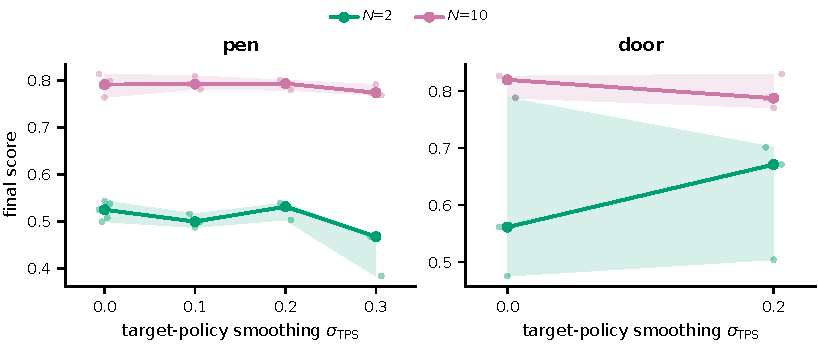
\includegraphics[width=.9\linewidth]{fig_tps.pdf}
  \caption{\textbf{Target-policy smoothing dose--response.} Final score vs.\
  $\sigma_{\mathrm{TPS}}$ at $N{=}2$ and $N{=}10$ ($M{=}2$, no dropout;
  median, min--max over 3 seeds; $\sigma_{\mathrm{TPS}}{=}0$ baselines from
  the main grid). TPS adds zero ensemble diversity; a small-$N$-specific gain
  is what the smoothness account predicts and what a diversity account has no
  mechanism for.}
  \label{fig:tps}
\end{figure}

\subsection{Sharpness as a prospective signal}
\label{sec:prospective}

Everything above is concurrent measurement. The practical question is whether
$\nsharp$ \emph{forecasts}: can a practitioner probe at an early checkpoint and
select configurations without finishing the grid? Across pen configurations,
$\nsharp$ at the 100k checkpoint (10\% of training) predicts final score with
$\rho_s{=}\ProspectiveRho{}$ ($n{=}\ProspectiveN$ runs; leave-one-config-out
range \ProspectiveLoco; excluding the divergent $M{=}1$ arms
$\rho_s{=}\ProspectiveRhoExclM$), and Fig.~\ref{fig:prospective} traces the
full horizon: the signal is present early and stabilizes. The probe costs
$\sim$$10^5$ critic forward passes --- free relative to a single training run
--- and requires no checkpoints, only logging.

\begin{figure}[t]
  \centering
  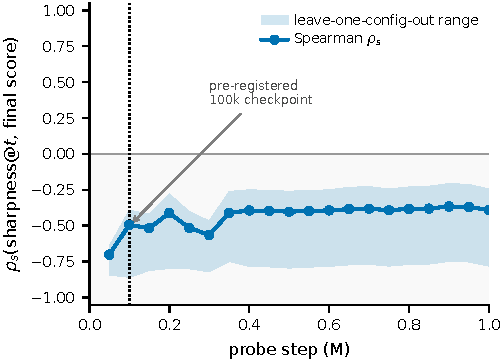
\includegraphics[width=.62\linewidth]{fig_prospective.pdf}
  \caption{\textbf{Early sharpness predicts final score.} Spearman
  $\rho_s\big(\nsharp\text{ at }t,\ \text{final score}\big)$ across pen
  configurations and seeds, vs.\ probe step $t$; band = leave-one-config-out
  range. Dotted line: the 100k checkpoint quoted in the text.}
  \label{fig:prospective}
\end{figure}

\section{Related work}
\label{sec:related}

Critic ensembles entered value-based RL for variance reduction
\citep{anschel2017averaged}; REDQ \citep{chen2021redq} scaled them to high
UTD continuous control with random $M$-of-$N$ minimization; DroQ
\citep{hiraoka2022droq} replaced most heads with dropout; RLPD
\citep{ball2023efficient} carried the recipe to offline-to-online learning
(cf.\ also \citep{song2023hybrid}) and reported dropout's null effect at
$N{=}10$. Diversity-centric accounts --- MSG's independent targets
\citep{ghasemipour2022msg}, EDAC's gradient diversification
\citep{an2021edac}, SPQR's independence regularizer \citep{lee2023spqr} ---
treat head disagreement as the explanatory variable; our measurements separate
disagreement from the smoothness of the mean and find score follows the
latter. Sharpness as flatness-of-minima is classical in generalization
\citep{keskar2016large,foret2021sam}; we transport it from parameter space to
the action space the actor differentiates. Spectral normalization bounds
critic Lipschitz constants globally \citep{bjorck2021spectral}; our
preliminary single-seed spectral-norm probes (App.~\ref{app:spectral}) were
confounded with LayerNorm and are superseded here by target-policy smoothing
\citep{fujimoto2018td3} as the controlled smoothness intervention.

\section{Limitations and conclusion}
\label{sec:conclusion}

\textbf{Limitations.} (i) Sharpness is probed on a fixed offline batch,
not at $(s,\pi(s))$ along the actor's own trajectory; the actor-side link ---
e.g.\ agreement of $\nabla_a\Sbar$ across heads at on-policy actions --- is
measured indirectly at best, and closing it is the clearest next experiment.
(ii) Scope is sparse-reward Adroit, where critic artifacts dominate; in
preliminary dense-reward runs (halfcheetah, single-seed, earlier harness) RLPD
saturates regardless of configuration, leaving no headroom for any account to
explain. (iii) Three to five seeds support sign-test-level claims, not effect
sizes. (iv) Sharpness is one mechanism among several: it does not by itself
explain the residual gap between $N{=}2{+}$dropout and $N{=}10$ at matched
$\nsharp$, nor interact with exploration.

\textbf{Conclusion.} The ensemble in RLPD is best understood not as a
pessimism device and not as a diversity device, but as a smoother of the one
function the actor touches: $\Sbar$. That reading unifies dropout's
small-$N$ gains and large-$N$ inertness as one saturation curve, survives a
normalization that removes the $Q$-scale confound, makes a falsifiable
prediction under an ensemble-free smoothing intervention
(\S\ref{sec:interventions}), and yields a free early-selection signal. The natural next target is flow-based offline-to-online methods such
as FQL \citep{park2025flow}, where ensembles are replaced by structured
critics: if the smoothness account is right, $\nsharp$ should predict
performance there without any ensemble in sight.

\bibliographystyle{plainnat}
\bibliography{refs}

\clearpage
\appendix

\section{Full results tables}
\label{app:tables}

\begin{table}[h]
\centering
\caption{Final score (fraction of horizon in success; median (min--max; $n$))
across the grid. Auto-generated; \pendingnum{} = awaiting fleet completion.}
\label{tab:headline}
\small
% AUTO-GENERATED by analysis/make_tables.py -- do not edit by hand
\begin{tabular}{llccc}
\toprule
env & $N$ & no dropout & dropout $p$=0.01 & $\Delta$ (median) \\
\midrule
pen & 2 & 0.53 \textsuperscript{(n=1)} & 0.75 \textsuperscript{(n=1)} & \pendingnum{} \\
pen & 4 & 0.69 \textsuperscript{(n=1)} & 0.79 \textsuperscript{(n=1)} & \pendingnum{} \\
pen & 6 & 0.77 \textsuperscript{(n=1)} & 0.77 \textsuperscript{(n=1)} & \pendingnum{} \\
pen & 10 & 0.81 \textsuperscript{(n=1)} & 0.78 \textsuperscript{(n=1)} & \pendingnum{} \\
pen ($M$=1) & 2 & 0.00 \textsuperscript{(n=1)} & 0.60 \textsuperscript{(n=1)} & \pendingnum{} \\
\midrule
door & 2 & 0.56 \textsuperscript{(n=1)} & \pendingnum{} & \pendingnum{} \\
door & 4 & 0.83 \textsuperscript{(n=1)} & \pendingnum{} & \pendingnum{} \\
door & 6 & 0.76 \textsuperscript{(n=1)} & \pendingnum{} & \pendingnum{} \\
door & 10 & \pendingnum{} & \pendingnum{} & \pendingnum{} \\
\bottomrule
\end{tabular}

\end{table}

\begin{table}[h]
\centering
\caption{Pre-registered contrasts. Seed pairs are same-seed, same-harness
dropout contrasts; config directions take one unit per $(env,N)$ cell;
$p$-values are exact two-sided binomial sign tests.}
\label{tab:signtests}
\small
% AUTO-GENERATED by analysis/make_tables.py
\begin{tabular}{lccc}
\toprule
contrast & positive / pairs & config directions & sign-test $p$ \\
\midrule
dropout $>$ none (pen) & 3/4 & 3/4 $N$-configs & 0.625 \\
dropout $>$ none (door) & \pendingnum{} & \pendingnum{} & \pendingnum{} \\
dropout $\Delta$ at $N$=2 (pen) & 0.22 \textsuperscript{(n=1)} & & \\
dropout $\Delta$ at $N$=10 (pen) & -0.03 \textsuperscript{(n=1)} & & \\
$N$=10 $>$ $N$=2 (no drop, both envs) & 1/1 & & 1.000 \\
\bottomrule
\end{tabular}

\end{table}

\begin{table}[h]
\centering
\caption{Prospective prediction: Spearman $\rho_s(\nsharp[0.05]\text{ at }t,$
final score$)$ across pen runs, with leave-one-config-out (LOCO) range, and
excluding the divergent $M{=}1$ arms.}
\label{tab:prospective}
\small
% AUTO-GENERATED by analysis/make_tables.py
\begin{tabular}{lcccc}
\toprule
probe step & $\rho_s$ (all) & LOCO range & $\rho_s$ (excl. $M$=1) & $n$ runs \\
\midrule
50k & -0.70 & [-0.84, -0.64] & -0.79 & 38 \\
100k & -0.49 & [-0.86, -0.39] & -0.82 & 38 \\
200k & -0.41 & [-0.80, -0.28] & -0.74 & 38 \\
500k & -0.40 & [-0.79, -0.26] & -0.73 & 38 \\
\bottomrule
\end{tabular}

\end{table}

\begin{table}[h]
\centering
\caption{Target-policy smoothing arm (median (min--max; $n$)). TPS runs are
never seed-paired with baselines (extra RNG split): distribution comparisons
only.}
\label{tab:tps}
\small
% AUTO-GENERATED by analysis/make_tables.py
\begin{tabular}{llcccc}
\toprule
env & $N$ & $\sigma_{TPS}$=0 & 0.1 & 0.2 & 0.3 \\
\midrule
pen & 2 & 0.53 (0.50--0.54; n=5) & 0.50 (0.49--0.52; n=3) & 0.53 (0.50--0.54; n=3) & 0.47 (0.38--0.47; n=3) \\
pen & 10 & 0.79 (0.76--0.81; n=5) & 0.79 (0.78--0.81; n=3) & 0.79 (0.78--0.80; n=3) & 0.77 (0.77--0.79; n=3) \\
door & 2 & 0.56 (0.48--0.79; n=3) & -- & 0.67 (0.50--0.70; n=3) & -- \\
door & 10 & 0.82 (0.79--0.83; n=3) & -- & 0.79 (0.77--0.83; n=3) & -- \\
\bottomrule
\end{tabular}

\end{table}

\section{Learning curves and $M{=}1$ diagnostics}
\label{app:curves}

\begin{figure}[h]
  \centering
  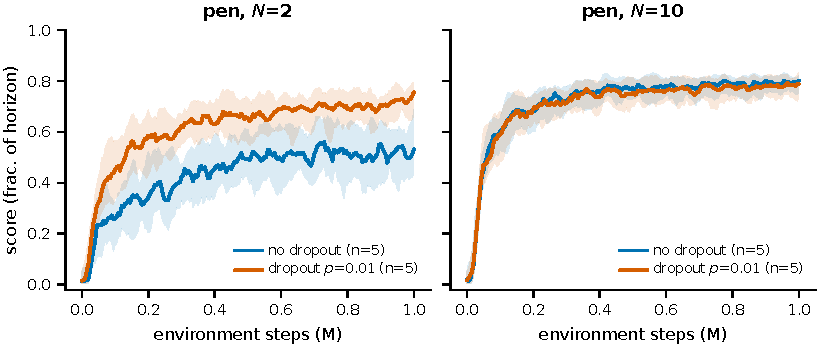
\includegraphics[width=\linewidth]{fig_curves.pdf}
  \caption{Pen learning curves (median, min--max band over seeds): $N{=}2$
  (left) and $N{=}10$ (right), with and without dropout.}
  \label{fig:curves}
\end{figure}

\begin{figure}[h]
  \centering
  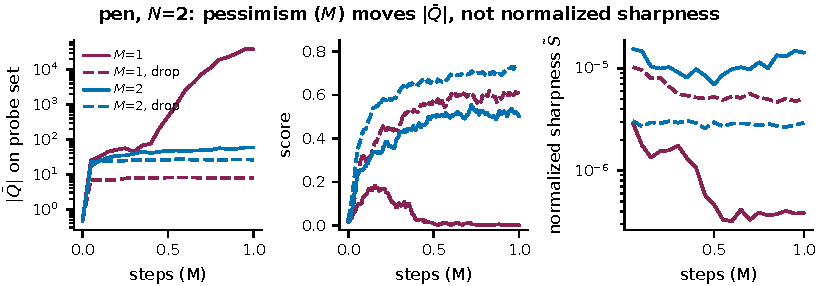
\includegraphics[width=\linewidth]{fig_minq.pdf}
  \caption{Min-$Q$ subsetting at $N{=}2$ on pen: $M{=}1$ (no min) blows up
  $|\Sbar|$ on the probe batch (left, log) and collapses score (middle),
  while normalized sharpness (right) separates the arms far less than
  amplitude does --- pessimism is amplitude control, not geometry control.}
  \label{fig:minq}
\end{figure}

\section{Perturbation-scale robustness}
\label{app:sigma}

\begin{figure}[h]
  \centering
  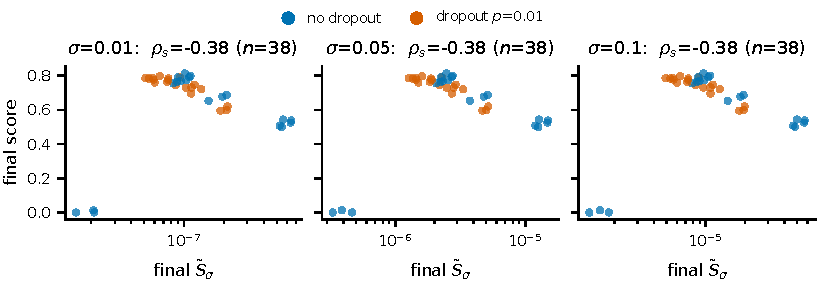
\includegraphics[width=\linewidth]{fig_sigma_robust.pdf}
  \caption{Final $\nsharp$ vs.\ final score at probe scales
  $\sigma\in\{0.01,0.05,0.1\}$ (independent perturbation seeds per scale).
  The association and config ordering are stable across scales; the course
  report's fixed $\sigma{=}0.05$ was not load-bearing.}
  \label{fig:sigma}
\end{figure}

\section{Cross-era replication check}
\label{app:replication}

The course-report era (April 2026) ran a near-identical grid single-seed on a
different cluster with a probe-free harness; those numbers are quarantined
from all claims. As a sanity check, seed-0 of the new fleet falls within (or
adjacent to) the new multi-seed bands and matches the April ordering:

\begin{table}[h]
\centering
\small
% AUTO-GENERATED by analysis/make_tables.py
\begin{tabular}{lccc}
\toprule
config (pen) & April (n=1 era) & June fleet & consistent? \\
\midrule
$N$=2, $M$=2, $p$=0.0 & 0.55 & 0.53 (0.50--0.54; n=5) & \checkmark \\
$N$=4, $M$=2, $p$=0.0 & 0.71 & 0.68 (0.65--0.69; n=3) & \checkmark \\
$N$=6, $M$=2, $p$=0.0 & 0.78 & 0.77 (0.76--0.77; n=3) & \checkmark \\
$N$=10, $M$=2, $p$=0.0 & 0.79 & 0.79 (0.76--0.81; n=5) & \checkmark \\
$N$=2, $M$=2, $p$=0.01 & 0.72 & 0.73 (0.70--0.75; n=5) & \checkmark \\
$N$=10, $M$=2, $p$=0.01 & 0.79 & 0.79 (0.76--0.80; n=5) & \checkmark \\
$N$=2, $M$=1, $p$=0.0 & 0.01 & 0.00 (0.00--0.01; n=3) & \checkmark \\
\bottomrule
\end{tabular}

\end{table}

\section{Diversity metrics}
\label{app:diversity}
% [FINALIZE] after /compare-runs: one paragraph + (optionally) the head/mask
% variance figure regenerated from diagnostic-era data or fleet mean_q logs,
% making the "diversity co-moves only through sharpness" claim quantitative
% (partial correlation of head_var with score given sharpness).
Measured head/mask variance comes from the earlier single-seed diagnostic
runs (April era, App.~\ref{app:replication} quarantine applies); the
dissociation argument in \S\ref{sec:sharp} therefore rests on the
\emph{designed} diversity contrasts, not on these measurements. In those
diagnostics, head variance falls with $N$ and mask variance appears only with
dropout, as expected by construction; across the configurations where diversity and
$\nsharp$ decouple ($N{=}10{+}$dropout: diversity up, $\nsharp$ flat, score
flat; $N{=}2{+}$dropout vs.\ $N{=}10$: diversity very different, $\nsharp$ and
score similar), score follows $\nsharp$.

\section{Preliminary spectral-norm probes (superseded)}
\label{app:spectral}

The course report attempted spectral normalization of critic layers
($\Sbar\mapsto$ scaled weights $w\,W/\sigma_{\max}(W)$) as a smoothness
intervention. Those runs were single-seed and structurally confounded:
LayerNorm (which RLPD requires) re-normalizes activations after the spectral
scaling, $w{=}0.5$ vs.\ $1.0$ dissociated sharpness from score, and the dense
reward replication did not move sharpness at all. We report this for
completeness and rely on target-policy smoothing --- which composes cleanly
with LayerNorm --- as the controlled intervention in this paper. A
LayerNorm-free spectral sweep remains future work.

\section{Reproducibility}
\label{app:repro}

JAX implementation on the reference RLPD codebase; single RTX 4000 Ada (20GB)
per run, 3.5--5.7 wall-hours per 1M-step run. Probe overhead $<\!1\%$.
All analysis (tidy tables, every figure and number in this paper) regenerates
from logs with one script; the pre-registered statistical discipline is
version-controlled alongside the harness. Code and logs released on
acceptance.
% [FINALIZE] add repo URL + commit hash at submission.

\end{document}
